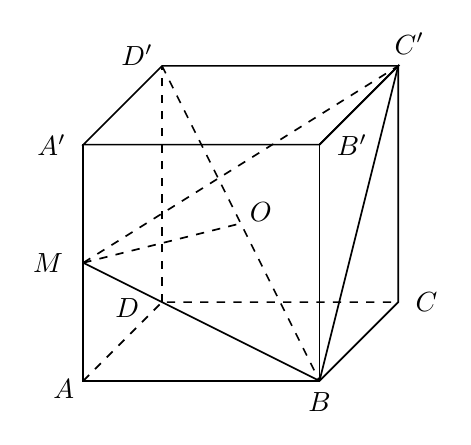
\begin{tikzpicture}[x=1cm,y=1cm,font=\normalsize,line width=.6pt]
\coordinate (A) at (0.00,0.00);
\coordinate (B) at (3.00,0.00);
\coordinate (C) at (4.00,1.00);
\coordinate (D) at (1.00,1.00);
\coordinate (Ap) at (0.00,3.00);
\coordinate (Bp) at (3.00,3.00);
\coordinate (Cp) at (4.00,4.00);
\coordinate (Dp) at (1.00,4.00);
\coordinate (M) at (0.00,1.50);
\coordinate (O) at (2.00,2.00);
% front face
\draw[solid] (A) -- (B) -- (Bp) -- (Ap) -- cycle;
% top face
\draw[solid] (Ap) -- (Bp) -- (Cp) -- (Dp) -- cycle;
% right face diagonals/edges
\draw[solid] (B) -- (C) -- (Cp) -- (Bp);
\draw[solid] (B) -- (Cp);
\draw[solid] (M) -- (B);
% hidden edges
\draw[dashed] (A) -- (D) -- (C);
\draw[dashed] (D) -- (Dp);
\draw[dashed] (Dp) -- (B);
\draw[dashed] (M) -- (Cp);
\draw[dashed] (M) -- (O);
\node[inner sep=2pt,below=3pt,left=1pt] at (A) {$A$};
\node[inner sep=2pt,below=2pt] at (B) {$B$};
\node[inner sep=2pt,right=4pt] at (C) {$C$};
\node[inner sep=2pt,left=2pt,xshift=-4.00bp,yshift=-2.00bp] at (D) {$D$};
\node[inner sep=2pt,left=4pt] at (Ap) {$A'$};
\node[inner sep=2pt,right=4pt] at (Bp) {$B'$};
\node[inner sep=2pt,right=4pt,above=2pt] at (Cp) {$C'$};
\node[inner sep=2pt,above=4pt,left=1pt] at (Dp) {$D'$};
\node[inner sep=2pt,left=5pt] at (M) {$M$};
\node[inner sep=2pt,above=4pt,right=1pt] at (O) {$O$};
\end{tikzpicture}
